\documentclass[a4paper]{article}
\usepackage[colorlinks=true,allcolors=blue]{hyperref}
\usepackage{amsmath}
\usepackage{graphicx}
\usepackage{amsfonts}
\usepackage[none]{hyphenat} %this is not necessary for the students to figure out, but a good thing to know
% it also sometimes gets rid of the overfull/underfull box warning



\title{Tables exercise}
\author{Me, myself and I}
\date{\today}

\begin{document}


\maketitle
	
\section*{Tables}
\subsection*{Exercise 1}

\noindent Let's first try our hand at a table containing some notable novels. The information on the country and year of publication comes from \href{https://en.wikipedia.org/wiki/Main_Page}{Wikipedia}.\footnote{Use the \textit{hyperref} package to add links to your document and add \texttt{[colorlinks=true,allcolors=blue]} before the package name to make all links and references blue.}

\begin{center}
\begin{tabular}{||l | l | l | l ||} 
 \hline
 \textbf{Title} & \textbf{Author} & \textbf{Country} & \textbf{Year}\\ [1mm] 
 \hline
 \hline 
 The Tale of Genji & Murasaki Shikibu & Japan & Before 1021 \\  
 \hline
 Journey to the West & Wu Cheng'en & Ming China & c. 1592 \\
 \hline
 Pride \& Prejudice & Jane Austen & England & 1813 \\ 
 \hline
 War \& Peace & Leo Tolstoy & Russia & 1865-67 \\
 \hline
  The Great Gatsby & F. Scott Fitzgerald & United States & 1925 \\
 \hline
\end{tabular}
\end{center}

\newpage

\subsection*{Exercise 2}
Recreate the following table in a style of your choice. Table taken from \href{https://www.unibas.ch/en/University/About-University/Facts-Figures.html}{Facts \& Figures page} of the Uni Basel.\\

\begin{figure}[h!]
    \centering
    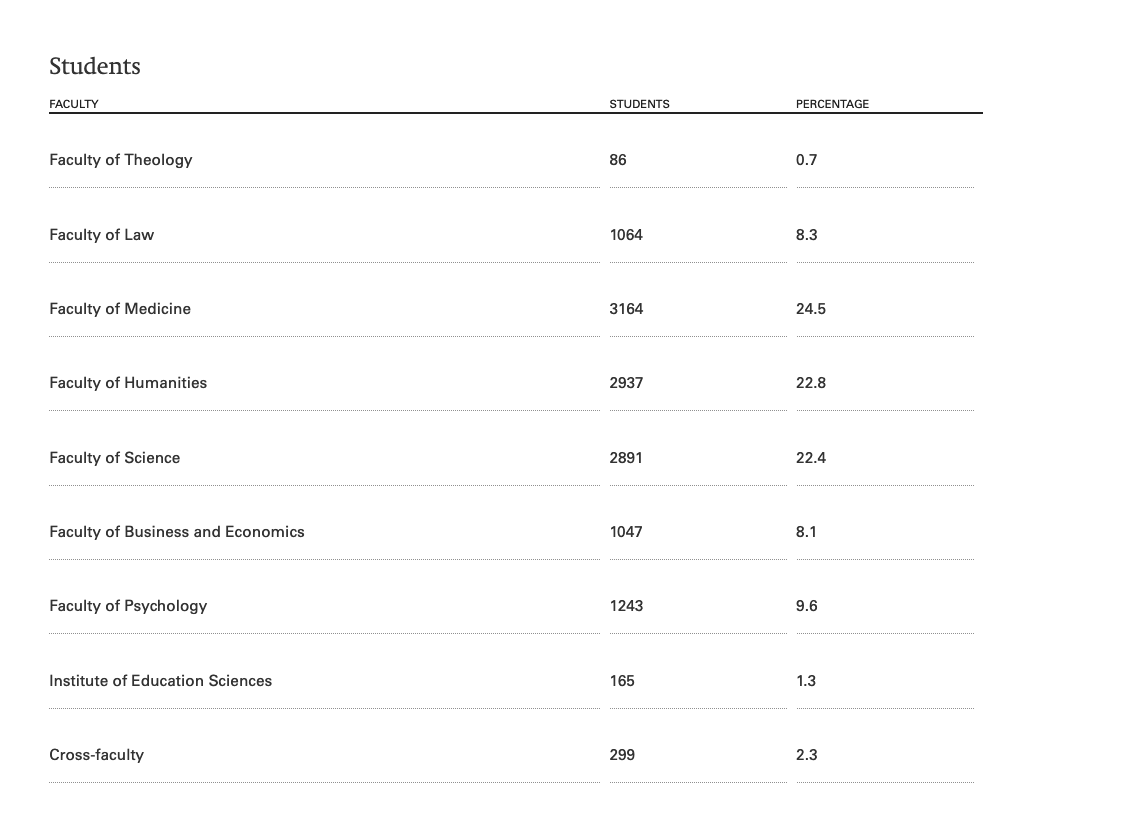
\includegraphics[width=\textwidth]{number_of_students.png}
\end{figure}
		
\end{document}